\begin{center}
  
  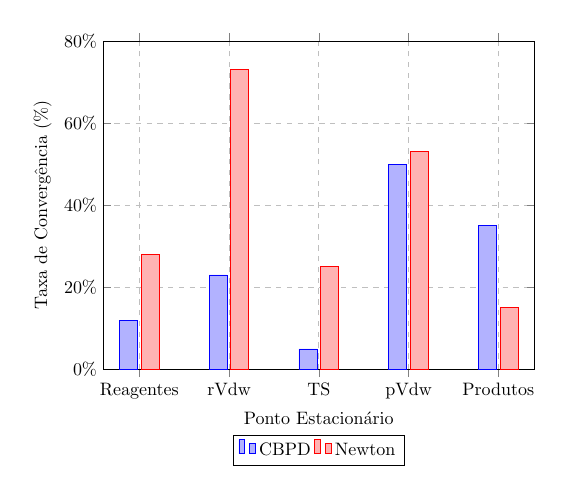
\begin{tikzpicture}[scale = 0.65]
    \begin{axis}[
      width=10cm,
      height=8cm,
      xlabel={Ponto Estacionário},
      ylabel={Taxa de Convergência (\%)},
      xtick=data,
      xticklabels={Reagentes, rVdw, TS, pVdw, Produtos},
      legend style={at={(0.5,-0.2)}, anchor=north, legend columns=-1},
      ymin=0,
      ymax=80,
      grid=major,
      grid style=dashed,
      ymajorgrids=true,
      ybar,
      ytick={0,20,...,80},
      yticklabel={\pgfmathprintnumber{\tick}\%}
    ]

      \addplot[color=blue, fill=blue!30] coordinates {
        (1, 12)
        (2, 23)
        (3, 5)
        (4, 50)
        (5, 35)
      };

      \addplot[color=red, fill=red!30] coordinates {
        (1, 28)
        (2, 73)
        (3, 25)
        (4, 53)
        (5, 15)
      };

      \legend{CBPD, Newton}

    \end{axis}
  \end{tikzpicture}

\end{center}
